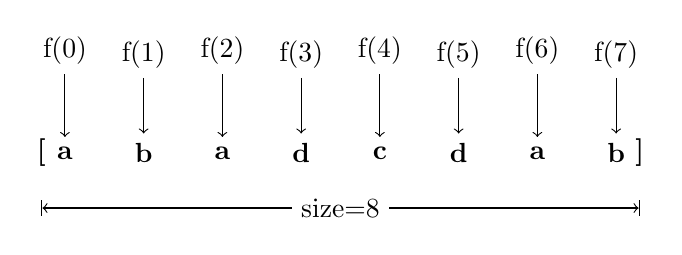
\begin{tikzpicture}

\foreach \i/\j in%
    {0/a,
     1/b,
     2/a,
     3/d,
     4/c,
     5/d,
     6/a,
     7/b} {
  \node (n_\i) at (\i, 0) {\textbf{\j}};
  \node (f_\i) at ([yshift=15mm]n_\i.south) {f(\i)};
  \draw[->] (f_\i) -- (n_\i);
}

\node[left of=n_0, xshift=0.7cm] (sqleft) {\textbf{[}};
\node[right of=n_7, xshift=-0.7cm] (sqright) {\textbf{]}};
\draw[|<->|] ([yshift=-4mm]sqleft.south) -- node[fill=white]{size=8} ([yshift=-4mm]sqright.south);
% \draw[|<->|] ([yshift=-4mm]n_0.south) -- node[fill=white]{size=8} ([yshift=-4mm]n_7.south);

\end{tikzpicture}
